\chapter{Spatial extensions to \stochsim{}}\label{spatial_extensions}

The original version of \stochsim{} (1.0) treated the entire reaction
system as a uniformly mixed solution.  Although this is clearly not
how molecules are arranged within living cells, the omission of spatial
heterogeneity has been a norm in biochemical simulations because it
greatly facilitates modelling and reduces the computational load of
simulation.  However, as the resolution of our understanding of
biochemical processes increases, it is becoming clear that even in
bacteria, the simplest of cells, the spatial organisation of molecules
often play an important role.  We have therefore undertaken extending
\stochsim{} to incorporate a spatial representation.

In versions of \stochsim{} later than 1.2, a simple two-dimensional
spatial structure is implemented, in which nearest-neighbour
interactions of molecules (such as clustered receptors on a membrane)
can be simulated.  This was motivated by studies of the bacterial
chemotaxis receptor complex which suggested that signal amplification
could be achieved in this complex if lateral interactions between
neighbouring receptors exist (Bray et al, 1998; Duke \& Bray, 1999).
The original implementation of this spatial structure only allowed
geometries composed of square units with four nearest neighbours, but
as of version 1.4, two additional geometries, one composed of
triangles and the other of hexagons, are supported.  These three are
the only three regular tesselations which can cover a two-dimensional
surface.  The new geometries can be used, for example, to reflect the
recent predection of the structural arrangement of the chemotaxis
receptor complex (Shimizu et al, 2000).

This chapter will describe how to use \stochsim{} \CURRENTVERSION{}
and later versions in order to simulate nearest-neighbour interactions
in a two-dimensional lattice.  Note that at present, GUI support for
specifying parameters specific to this spatial structure is still
incomplete.  The user is therefore required to write one of the
configuration files by hand.  However, most simulation parameters can
now be written using the Perl/Tk GUI.

\section{Overview}\label{se_overview}

In addition to the standard configuration files (documented in Chapter
\ref{conf_files}), at least two additional configuration files must be
set up for \stochsim{} simulations using the 2-D complex arrays.  The
first file is the complex array file (usually named
\texttt{ARRAY.INI}).  This file specifies the number of complex arrays
to be used, their names, dimensions, their component complex types, as
well as several other options.  The formatting of this file is not yet
supported in the GUI, so it must be written by hand.  At present, each
array can contain only one complex type, which must be a
\textbf{neighbour-sensitive complex (NS-Complex)}.  For each type of
NS-Complex used in the simulation, an additional configuration file
(usually named \texttt{NS\_\emph{X}.INI}, where \emph{X} is a number)
must be defined, which specifies the details of its behaviour.  The
neighbour-sensitive configuration files can now be set up using the
Perl/Tk GUI.

NS-Complexes are similar to multistate complexes, but can additionally
take part in \textbf{neighbour-sensitive reactions (NS-Reactions)} and
\textbf{neighbour-sensitive rapid equilibria (NS-RapidEqm's)}.  These
are similar to multistate reactions and rapid equilibria, but the
actual reaction rate or rapid equilibrium probability depends not only
on the state of the chosen complex, but also on the states of its
nearest neighbours within the complex array.  The NS-Reactions and
NS-RapidEqm's are defined within the neighbour-sensitive configuration
file for each NS-Complex.  Of course, NS-Complexes can take part in
normal \stochsim{} reactions and RapidEqm's which are not sensitive to
the state of neighbours.  These are defined as usual in the standard
configuration files \texttt{REACTION.INI} and
\texttt{MS\_\emph{X}.INI}.

The primary purpose of this spatial structure implementation so far
has been to study various properties of complex arrays of fixed size
and geometry.  Therefore, it does not presently support movement of
NS-Complexes, neither between nodes within the array or into and out
of the array.  The binding of other complexes in the reaction system
to complexes within the complex array is permitted, but does not alter
the size or geometry of the array.  In all complex arrays, each node
has exactly one complex.  Each node in turn has three, four or six
nearest-neighbour nodes, depending on the geometry of the array, which
can be made up of either triangles, squares or hexagons (see Figure
\ref{fig-geometry}).  Boundaries can be either real (i.e. nodes at
the edges of the array have fewer neighbours) or toroidal (i.e. a
coordinate system representing a doughnut shape; nodes at the opposite
extremity of each axis are treated as nearest neighbours).

\begin{figure}
\begin{center}
\begin{tabular}{ccc}
\scalebox{0.27}{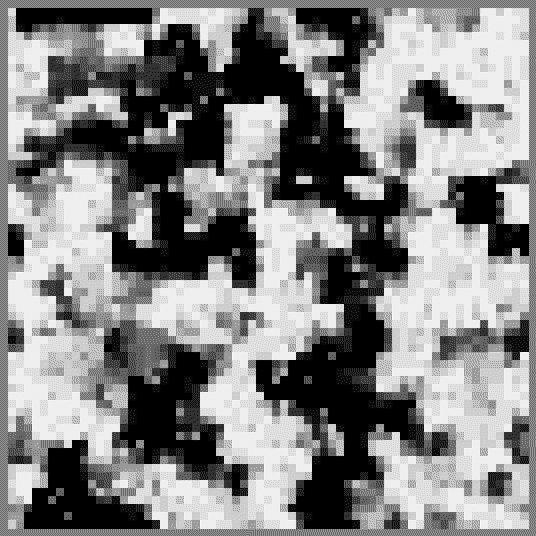
\includegraphics{array_snapshot_square.jpg}} &
\scalebox{0.27}{
\includegraphics{array_snapshot_trig.jpg}} &
\scalebox{0.27}{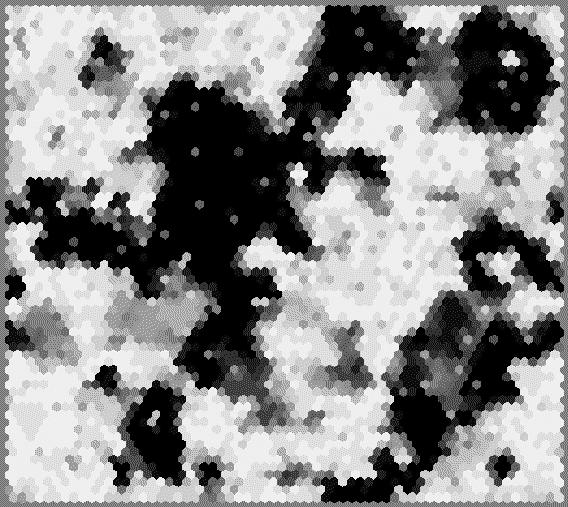
\includegraphics{array_snapshot_hex.jpg}}\\
(a) & (b) & (c)
\end{tabular}
\caption{The complex arrays in \stochsim{} 1.4 can have geometries
  based on (a) squares, (b) triangles or (c) hexagons.  Images such as
  these can be generated from the snapshot output of \stochsim{} by
  using the script \texttt{arraydraw.py} to generate images such as
  these.}
\end{center}
\label{fig-geometry}
\end{figure}

\section{Setting up a simulation that uses 2-D complex arrays
  (\texttt{STCHSTC.INI})}

In order to tell the \stochsim{} program that 2-D complex arrays will be
used in a simulation, the following optional parameters must be
specified in the main simulation configuration file (\texttt{STCHSTC.INI}).

\subsection{[Options]}
\begin{description}
\item[UseSpatialExtensions] This parameter specifies whether or not
  \stochsim{}'s spatial extensions will be used in a simulation.  This
  value must be set to 1 when using 2-D complex arrays. When this is
  set to 0, \stochsim{} ignores the following two parameters and behaves
  exactly like \stochsim{} 1.0.
\end{description}

\subsection{[File Names]}
\begin{description}
\item[ArrayINIFile] The path name specifying the location of the
  complex array configuration file (e.g. ``\texttt{./ARRAY.INI}'').
  
\item[ArrayOutPrefix] A path name which will be the prefix of all
  array output files (e.g. ``\texttt{../Output/}'').  The final name
  of each complex array output file (e.g. \\
  ``\texttt{../Output/ARRAY\_SNAPS\emph{X}.OUT}'') will consist of a suffix
  appended to this prefix.
\end{description}



\section{Definition of complex arrays (\texttt{ARRAY.INI})}\label{array_ini}

The complex array configuration file can take any name, as long as it
matches the name specified in the simulation configuration file, but
we recommend using something fairly obvious (e.g.
``\texttt{ARRAY.INI}'').  This file consists of three or more
sections: one \textbf{[General]} section, one \textbf{[Neighbour
  Sensitive Complex Types]} section\footnote{As of version 1.4, the
  preferred location of this section is in the complex configuration
  file (\texttt{COMPLEX.INI}).}, one or more
\textbf{[\emph{ARRAY\_NAME}]} (where \emph{ARRAY\_NAME} is the name of
the array) sections, and zero or more \textbf{[Snapshot Variable
  \emph{X}]} (where \emph{X} is a number) sections.  An
\textbf{[\emph{ARRAY\_NAME}]} section must be defined for each complex
array to be used in the model, and a \textbf{[Snapshot Variable
  \emph{X}]} section must be defined for each snapshot output that is
desired (see section \ref{se_output}). The parameters which must be
specified in each section are as follows:

\subsection{[General]}
\begin{description}
\item[Arrays] The list of complex arrays to be used.  The name of each
  array must be given here as a comma-separated list.
  
\item[DumpInterval] The interval between times at which complex array
  dumps should be stored (floating point).

\item[NumSnapshotVariables] The number of snapshot variables that are
  defined in this file (integer).
\end{description}

\subsection{[Neighbour Sensitive Complex Types]}
Note that as of version 1.4, the preferred location of this section is
in the complex configuration file (\texttt{COMPLEX.INI}).  If it is
defined in both files, the definition in the complex array
configuration file (\texttt{ARRAY.INI}) will be ignored.

\begin{description}
\item[NeighbourSensitiveComplexes] A comma-separated list of symbols,
  one for each neighbour-sensitive complex type in the reaction
  system.
  
\item[\emph{S}\_NS\_INIFile] For each NS-Complex type in the model, a
  line of the following form must be specified here:\\[\baselineskip]
  \emph{S}\_NS\_INIFile = \emph{Path}\\[\baselineskip]
  where \emph{Path} is the path name of the configuration file for the
  NS-Complex type \emph{S} (usually named \texttt{NS\_\emph{X}.INI},
  where \emph{X} is a number).
\end{description}

\subsection{[\emph{ARRAY\_NAME}]}
\begin{description}
\item[Complex] The name of the complex type that constitutes this
  complex array.
  
\item[NeighbourSensitive] Whether the complex type that constitutes
  this complex array is neighbour sensitive (must always be set to 1
  in present implementation).

\item[Geometry] The geometry of the complex array (must be one of
  ``Square'', ``Triangle'' or ``Hexagon'').

\item[BoundaryCondition] The boundary condition to be used for this
  complex array (0 = Toroidal, 1 = Real boundaries).

\item[XDimension] The length of the X-axis of the complex array (integer).

\item[YDimension] The length of the Y-axis of the complex array (integer).
  
\item[CreateDumpFile] Whether or not the state of this complex array
  should be dumped to a file during simulation (1 = Yes, 0 = No).
  Note that array dumps are different from array snapshots!
  
\item[EquilibrationInterval] The interval between times at which this
  complex array is to be equilibrated (floating point).  All rapid
  equilibria defined for each complex within the complex array will be
  equilibrated at this frequency.
\end{description}

\subsection{[Snapshot Variable \emph{X}]}
\begin{description}
\item[Array] The name of the array that this snapshot variable represents.
\item[States] A comma-separated list of bit strings (or wildcard
  strings) that represent all the states that this snapshot variable
  will represent.  It is convenient to use wildcard strings here, if
  you want to monitor the state of specific flags (e.g.  ``1?0?'', for
  a complex with four state flags when you want to highlight all
  complexes with the first flag on and the third flag off).
  
\item[StoreInterval] The interval between the times at which values
  of this snapshot variable are to be stored (floating point).

\item[AveragedOutput] Specifies whether snapshot output of array
  states should be be instantaneous or time-lapse (0 = instantaneous,
  1 = time-lapse).
  
\item[AverageInterval] If time-lapse snapshots are desired, give the
  length of the interval to use for averaging (floating point; must be
  smaller than value specified for \textbf{StoreInterval}).  This
  parameter is ignored if \textbf{AveragedOutput} is set to 0.
  
\item[SampleInterval] If time-lapse snapshots are desired, give the
  interval between times at which values should be sampled for
  averaging (floating point; must be smaller than value specified for
  \textbf{AverageInterval}).  This parameter is ignored if
  \textbf{AveragedOutput} is set to 0.
\end{description}

\section{Definition of neighbour-sensitive complexes (\texttt{NS\_\emph{X}.INI})}
\subsection{[General]}
\begin{description}
\item[NumRapidEqm] The number of state flags of this NS-Complex that
  are controlled by NS-RapidEqm's (integer).  Note that this number
  should only include the number of NS-RapidEqm's, and not normal
  RapidEqm's, which are be defined separately in the multistate
  complex configuration file (\texttt{MS\_\emph{X}.INI}).
  
\item[Reactions] A comma-separated list of reaction identifiers for
  NS-Reactions.  Be careful to use the same identifiers as specified
  in the reaction configuration file (\texttt{REACTION.INI}) and multistate
  configuration file.
  
\item[NumNeighbours] The number of nearest neighbours that this
  NS-Complex has in the complex array (integer). Note that
  this number must correctly match the geometry of the complex array
  that this NS-Complex will be inserted into (3 for ``Triangle'', 4
  for ``Square'' and 6 for ``Hexagon'').  
\end{description}

\subsection{[Rapid Equilibrium \emph{X}]}
Each NS-RapidEqm must have a section headed [Rapid Equilibrium
\emph{X}] where \emph{X} is the number of the rapid eqm
\begin{description}
\item[Flag] The name of the state flag which is controlled by an
NS-RapidEqm. ``State'' is also accepted for backward compatibility but
  is deprecated.
  
\item[CoupledStates] A comma separated list of wildcard strings (do
not use whitespaces), representing the states of nearest neighbours
that are coupled to this NS-RapidEqm.

\item[Wildcards] A comma-separated list of all bit strings below which
  contain one or more of the wildcard character, '?'. Wildcards
  represent \emph{both} 0 and 1.
  
\item[\emph{BitString}] Defines the NS-RapidEqm probabilities
  associated to specific states.  The parameter name,
  \emph{BitString}, can be a bit string representing a single state,
  or a wildcard string representing multiple states.  If wildcard
  strings are used, they must also be declared in the
  \textbf{Wildcards} parameter described above.  The probabilities
  defined in each line are applied only when the complex is in a state
  which matches that (those) specified in the parameter name.  The
  value of this parameter must be a comma separated list of
  rapid-equilibrium probabilities.  The number of probabilities in
  this list must be exactly \textbf{NumNeighbours} + 1. These
  correspond to the rapid-equilibrium probabilities of the flag
  (specified by the \textbf{Flag} parameter in this section) when
  zero to \textbf{NumNeighbours} neighbours are in a coupled state.
  Multiple instances of this line should be defined, if necessary.
  For states that are not defined here, a default probability of zero
  is assigned automatically.
\end{description}

\subsection{[Reaction \emph{XD}]}
Each reaction involving a NS-Complex must have a section [Reaction
\emph{XD}] where X is the reaction number and D is direction ('F' or
'R').
\begin{description}
\item[ReactNeighbourID] A numerical identifier specifying the reacting
  neighbour (e.g. for the ``Square'' geometry, 0 = North, 1 = East, 2
  = South, 3 = West).

\item[EffectOnNeighbour] A comma-separated list of state changes on
the reacting neighbour resulting from this reaction.  A '+' character
before the name of the affected flag indicates that the flag is set (0
-> 1); a '-' character indicates that the flag is cleared (1 -> 0);

\item[Wildcards] A comma-separated list of all bit strings below which
  contain one or more of the wildcard character, '?'. Wildcards
  represent \emph{both} 0 and 1.

\item[\emph{BitString}] Defines the NS-Reaction relative rate
(floating point; 0 <= \emph{p} <= 1) associated to specific states.
The parameter name, \emph{BitString}, can be a bit string representing
a single state, or a wildcard string representing multiple states.
The probability defined in each line are applied only when the complex
is in a state which matches that (those) specified in the parameter
name.  Multiple instances of this line should be defined, if
necessary. For states that are not defined here, a default probability
of zero is assigned automatically.
\end{description}

\section{Output of complex-array states}\label{se_output} 

\subsection{A note for StochSim 1.2 users}
Before reading this section, please note that the way in which the
output of complex-array states are specified in the INI files has
undergone considerable changes between \stochsim{} 1.2 and 1.4.  In
this section we will only describe the new way of specifying the
output which only applies to \stochsim{} 1.4 and later.  If you are
still using \stochsim{} 1.2, we recommend that you upgrade to
\stochsim{} 1.4, which incorporates various new features and also has
been further optimised for speed.  However, if for some reason you
wish to keep using \stochsim{} 1.2, please refer to the older versions
of this manual.

\subsection{Array snapshots}
\stochsim{} 1.2 and later versions can output the state of an entire
complex array at any given time during simulation as graphical
representations called \emph{snapshots}.  In a snapshot, each
NS-Complex in the complex array is represented by a polygon
(corresponding to that specified for the array geometry\footnote{Note
  that in \stochsim{} 1.2, only the ``Square'' geometry was
  supported.}), so the entire image representing the array will be a
tesselation of polygons.  You can specify a single state
or a combination of states of the NS-Complex that you want highlighted
in the snapshot, so that the spatial distribution of specific states
that you are interested in can be visualised.

There are two types of snapshots that can be created,
\emph{instantaneous} and \emph{time-lapse} (see Figure
\ref{fig-snapshots}).  Instantaneous snapshots are snapshots in which
the instantaneous state of the complex array is recorded (i.e. the
value of each pixel is either 0 or 1).  Time-lapse snapshots are
snapshots in which the value of every pixel in the snapshot is
averaged over time (i.e. the value of each pixel is between 0 and 1).

\begin{figure}
\begin{center}
\resizebox{3.5cm}{3.5cm}{
\includegraphics{array_snapshot_inst.jpg}}
\hspace{1cm}
\resizebox{3.5cm}{3.5cm}{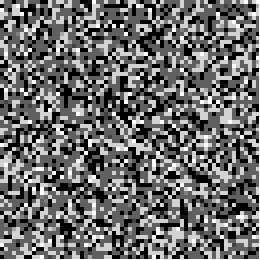
\includegraphics{array_snapshot_ave.jpg}}\\
(a) \hspace{4cm} (b)
\end{center}
\caption{\stochsim{} 1.2 and later versions can output
  (a) instantaneous snapshots, or (b) time-lapse snapshots of an array
  of NS-Complexes.  The tiled polygons of an instantaneous snapshot
  are either white or black.  The polygons of a time-lapse snapshot
  have grey level somewhere between white and black, depending on the
  proportion of time that the corresponding NS-Complex spent in the
  highlighted state.}
\label{fig-snapshots}
\end{figure}

In the instantaneous snapshots, white pixels represent NS-Complexes
which are in the highlighted state, and black pixels represent
NS-Complexes in all other states.  In the time-lapse snapshots, grey
levels are assigned to the pixels according to the proportion of time
each NS-Complex object has spent in the highlighted state (i.e.
NS-Complexes which were in the highlighted state 100\% of the time
will show up white, and NS-Complexes which were never in the
highlighted state will show up black).

Snapshots are recorded at a user-specified frequency during the
simulation.  Time series of snapshots are recorded in output files
named \texttt{ARRAY\_SNAPS\emph{X}.OUT}, where \texttt{\emph{X}} is a
numerical identifier for each series of snapshots.  Each file contains
snapshots with different highlighted states.  Each of these snapshot
files is essentially a concatenated series of X Pixmap (XPM) format
image files.  To view each snapshot, the snapshot file must be split
into separate image files.  As of version 1.4, a novel utility program
called \texttt{arrayview.py} for this purpose is providedin the
\texttt{bin} directory of the \stochsim{} distribution.  This program
can generate a series of GIF files from a StochSim snapshot file.  It
will also automatically determine the geometry of the array from the
snapshot file, and draw triangles, squares or hexagons as necessary
(see Figure \ref{fig-geometry}).  \texttt{arraydraw.py} is written in
Python, which works on just about all modern operating systems, and
comes installed as standard on most UNIX operatins systems these days.
To run \texttt{arrayview.py}, simply type
\\[\baselineskip]
\texttt{ \% arraydraw.py \emph{snapshot\_file} [edge\_length] }
\\[\baselineskip]
at the UNIX command-line. \texttt{[edge-length]} is an optional
argument which tells \texttt{arraydraw.py} how long you want the edges
of the polygon to be.  If you are using Microsoft Windows or a UNIX
operating system without python installed, you must first download and
install the python interpreter (available from
\url{http://www.python.org}).  Once the images have been generaged,
any image viewer can be used to view the images.

If you want to created animations from the image files, you can use
external programs such as \texttt{gifsicle} (available from
\url{http://www.lcdf.org/gifsicle/}), which can generate GIF
animations from a series of GIF image files.

\subsubsection{Example: How to set up the output of snapshots}
Let's say you have an array of receptors named ``ARRAY1''. The
NS-Complex which makes up this array has two state flags.  The first
flag, named ``L'', represents the state of the ligand binding site (1
= bound; 0 = unbound). The second flag, named ``X'', represents the
conformational state of the receptor (1 = active conformation; 0 =
inactive conformation).  Now, let us suppose that you want to monitor
both the changes in activity and ligand binding of all the receptors
in the array, averaged over time.  For this you will need two series
of time-lapse snapshots, one to monitor the activity, and one to
monitor the state of the ligand binding site.

To specify the snapshots you want, you must set up a \textbf{Snapshopt
  Variable} for each snapshot.  These are defined in the complex array
configuration file (\texttt{ARRAY.INI}).  Each snapshot variable must
be defined in its own \textbf{[Snapshot Variable \emph{X}]} section,
which has seven parameters (see section \ref{array_ini} for formatting
details).  The first five parameters must be defined for all snapshots
.  The first parameter, \textbf{Array} specifies the name of the array
that the snapshot variable will represent.  The next parameter,
\textbf{State} specifies the states of the NS-Complex that this
variable will highlight in the snapshot output, using a
  comma-separated list of bit strings (or wildcard strings).
\textbf{StoreInterval} specifies how often snapshots from this
variable are to be output during the simulation, and
\textbf{AveragedOutput} is a boolean parameter specifying whether or
not the output snapshots should be averaged over time (set to 1 if
averaging is desired, and 0 otherwise).  If \textbf{AveragedOutput} is
set to 1, the parameters \textbf{AverageInterval} and
\textbf{SampleInterval} must also be set.  \textbf{AverageInterval} is
the length of the interval over which the snapshot values will be
averaged, and \textbf{SampleInterval} is the inverval between times at
which values are sampled for averaging.  For this example, we will use
0.1 for the store and average intervals, and 0.001 for the sample
interval.  Note that the value of \textbf{AverageInterval} cannot be
larger than \textbf{StoreInterval}, and \textbf{SampleInterval} cannot
be larger than \textbf{AverageInterval}.

% When specifying \textbf{StoreInterval} and
% \textbf{AverageInterval}, the characteristic rates of whatever
% processes control the state changes being monitored should be
% considered (e.g. if the rate of a reaction controlling a certain flag
% is about 10 s\textsuperscript{-1}, you should set StoreInterval to
% smaller than 0.05).

So, for the example here, you would define two Snapshot Variables.
The two sections defining these variables would like this:
\begin{small}
\begin{verbatim}
[Snapshot Variable 1]    ;; Snapshot variables must be numbered sequentially
Array           = ARRAY1 ;; Specify the name of the array here
States          = 1?     ;; States matching this wildcard string are hi-lited
Name            = RL     ;; You can name variables as you like
StoreInterval   = 0.1    ;; Interval between storage times (s)
AveragedOutput  = 1      ;; Indicates whether output should be averaged
AverageInterval = 0.1    ;; Length of averaging interval (s)
SampleInterval  = 0.001  ;; How often values are sampled for averaging (s)

[Snapshot Variable 2]    
Array           = ARRAY1 
States          = ?1     
Name            = RX     
StoreInterval   = 0.1    
AveragedOutput  = 1      
AverageInterval = 0.1    
SampleInterval  = 0.001  
\end{verbatim}
\end{small}

The wildcard strings specified for the \textbf{State} parameters,
``1?'' (matches both ``10'' and ``11'') tells \stochsim{} to create a
series of snapshots that highlight NS-Complexes with the first flag on
(receptors with ligand bound), and ``?1'' (matches both ``01'' and
``11'') tells \stochsim{} to create another series of snapshots that
highlight NS-Complexes with the second flag on (active receptors).

That's it!  You should find two new output files after the
simulation, one named \texttt{ARRAY\_SNAPS1.OUT} (with the
ligand-bound receptors highlighted) and another named
\texttt{ARRAY\_SNAPS2.OUT} (with the active receptors highlighted).

\subsection{Array dumps}
As of version 1.4, \stochsim{} can output the complete state of the
complex array in ``dump files'' which can later be used to resume the
simulation from the time at which the state was dumped.  If such an
output is desired for an array, the parameter \textbf{CreateDumpFile}
in the \textbf{[\emph{ARRAY\_NAME}]} section must be set to 1.  The
frequency at which all array dumps will be output to dump files must
be specified using the parameter \textbf{DumpInterval} in the
\textbf{[General]} section of the complex array configuration file
(\texttt{ARRAY.INI}).

%\section{Manipulating the array output}
%       *monochrome
%       *colour

%%% Local Variables: 
%%% mode: latex
%%% TeX-master: "stochsim_manual"
%%% End: 
